% !TeX root = ../main.tex
% Add the above to each chapter to make compiling the PDF easier in some editors.

\chapter{Introduction}\label{chapter:introduction}


In this chapter we introduce the reader to the \textit{Context} of the topic, which is the manufacturing domain and the engineering approaches within the domain as well as the role of software tools and their impact on the engineering, so the reader would have a better understanding of the general area of the problems the thesis focuses on and their impact. Then we go into more details of the \textit{Engineering processes and tools} used in manufacturing engineering to show the specific scope of the thesis. In the \textit{Problem statement} section there is a description of the problem of evaluation of the tool-based engineering approaches used during the engineering processes the thesis solves.\textit{ Method and outline} gives an general view on the method of solving the problem and the outline of the thesis document for a comfortable navigation throughout the document.

\section{Context}
In the manufacturing domain, engineers work with complex systems that consist of components from a variety of disciplines, such as mechanics, electronics, informatics etc. As the development of manufacturing systems is a complex process, which furthermore needs to be fast, have a high efficiency and quality to fill the needs of the industry, there are a lot of techniques, studies and practices of how to make it meet the requirements of quality and speed and make it as efficient as possible. There is a potential for the improvement of the processes and different disciplines offer a plenty approaches for manufacturing development. \\

Informatics is one of the areas that can effect the methodology of the manufacturing engineering, as the majority of the work in the modern mechatronics is done with a help of a specific software or a set of different programs. Naturally the engineering tools, that are used during the development influence the engineering process. Software is already the main innovation driver in many industry branches \cite{russwurm}, thus there is a potential for improvement of the development approach accordingly to the software.\\

There are software solutions for the industrial engineering that influence the development process and approach of systems design. In this thesis we focus on software-based engineering approaches. Therefore what these solutions offer to the industry is a tool that either supports the traditional engineering practice, either offers changes to the process. \\

Manufacturing and industrial domains are rigid areas in the terms of embracement of the new technologies, because of the scope, risks and costs of changes. Thus there should be a strong reasoning in order to start the expensive, risky and complicated process of introducing a new software and project development methodology.
This is why it's important to have the means to evaluate the engineering approaches in order to find out whether they are good enough, fit the needs of the industrial enterprise and whether the advantages they claim to provide actually are worth the changes.  \\

  
\section{Engineering processes and tools}
According to \cite{kolk} the typical process of the development of a mechatronic project looks as on the Figure \ref{fig:mech_design}. Software tools are used on the stages 5 through 9 and help the engineers create, debug and optimize both mathematical and modular models and prototypes of the designed systems. Some examples of these tools are LabVIEW, Simulink/Matlab, Matrix-x, ACSL, Siemens Mechatronics Concept Designer, SimPACK, Hypersignal, and VisSim. These graphical simulation and prototypical tools run on generic platforms such as desktop PC compatible Windows, Linux or Mac OS operating systems \cite{shetty}.\\

 \begin{figure}[htb]
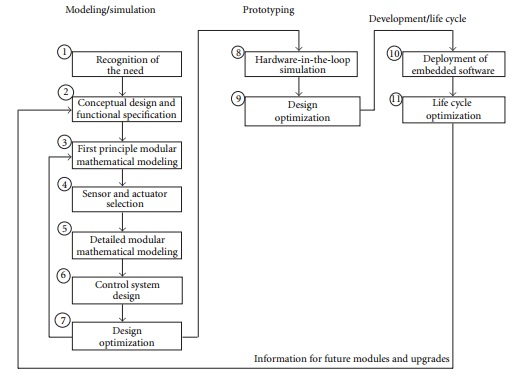
\includegraphics{figures/mech_design_process.jpg}
\caption{Mechatronics design process}
\label{fig:mech_design}
 \end{figure}

MaCon is an alternative development approach that offers to shift from mechanically dominated engineering principles to mechatronics development \cite{dese}. It provides a model-based method and prototypical tool (called the MaCon workbench) for interdisciplinary manufacturing system specification as well as continuous syntactic and frequent semantic quality assurance. In particular, the approach promotes top-down and test-driven conceptual design of a manufacturing system.\\

MaCon offers a model-based development approach, which means there is a common model of the system designed collaboratively by engineers within an interdisciplinary team. Thus the model provides a common understanding of the system to the whole development team and prevents the consistency problems by having the common basis at the early stage of the project development.\\

According to \cite{Hackenberg2016} nonetheless the model-based approach is well known it is not widely used in the area because of additional cost of model development. Although as the systems get more and more complex, the cost of the initial model design is overshadowed by the cost of consistency issues that appear on later stages of the process. The tendency of rising complexity of the systems is predicted to continue, thus there is a potential for the industry to embrace the model-based approach.\\ 

The approach offers the engineering process to consist of two phases: \textit{conception} and \textit{refinement}, as shown on the Figure \ref{fig:phases}.  During the first phase the common mechatronic concept is designed to capture the common understanding of the system. The concept includes the description of the system in the terms of requirements, common structure/architecture, approximate system behavior. Validation, verification and consistency checking are done via testing/simulation. \\

 \begin{figure}[htb]
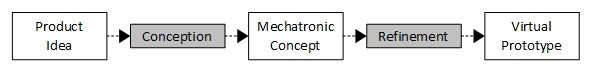
\includegraphics{figures/phases.jpg}
\caption{MaCon engineering process}
\label{fig:phases}
 \end{figure}
 
 During the refinement phase the complete virtual prototype is being build. After this phase the resulting prototype is supposed to contain all relevant documents for the manufacturing of the system. During the phase the engineers work of the details of the mechanical, electric/electronic and software aspects of the system. The development process during the refinement stage is supposed to be iterative with a constant use of testing/simulation for prototype verification. The entire process is supported by MaCon workbench.\\ 

\section{Problem statement} \label{section:problem}
The manufacturing domain is being offered multiple tool-based engineering approaches so the question is: "\textit{How to evaluate the tool-based engineering approaches?}"\\

The importance of the topic lies in the conflict between modern alternative approaches and conservative methods in manufacturing domain. Nonetheless the modern approaches promise more effective engineering, the industry tends to stick to the old methods. There should be means to prove the efficiency of the new methods in order for the industry to find it worthy the expensive and complicated changes it takes to embrace the new development approach. \\

This thesis focuses on evaluation of the engineering approaches on the example of the MaCon approach. Although the approach is a well-thought solution that has a great potential for the industry there are a lot of questions about how good the approach is, how efficient the tools the MaCon workbench offers are, what the potential weaknesses and ways to improve both approach and the workbench are. \\


Therefore the thesis is supposed to offer an evaluation solution for tool-based engineering approaches on the example of MaCon. The main goal of the evaluation process on the approaches is to either improve the approach, either to prove that it's a good solution for the industry.  \\

In this thesis we focus on the evaluation, that is based on the experiment, which is a user research and the following analysis of the experiment results. It involves a user study over the MaCon software and the following retrospective analysis of the data collected during the experiment. This thesis presents the detailed description of the experiment design, collected data and tool for the analysis. The MaCon approach as a tool-based engineering solutions is supposed to be evaluated as:
\begin{itemize}
\item engineering method in terms of efficiency of the method
\item modeling technique in terms of suitability of the model
\item prototyping tool in terms of usability of the tool
\end{itemize}

In order to perform the evaluation there need to be means to reconstruct the process, collect the user feedback, audio and video material and analyze both. Feedback includes ratings, multiple and single choice questions, as well as free form feedback, which altogether are a typical survey. The solution has to provide opportunity to process the feedback and extract knowledge out of it. Audio and video material includes microphone recording to capture discussions, oral feedback etc., screencast to capture interaction with the workbench and other tools, like browser and others, webcam recording to capture participant's reaction, whiteboard, etc. For process reconstruction there should be means to mark certain events or states, therefore there should be functionality to leave bookmarks and connect them to the recordings. The data collection has to be process-sensitive, which means it has to react to certain events, usage patterns or states of the project, for example the researcher might be interested in situations, when the usage of the system doesn't fit to the expected behavior, like if the requirements objects are edited outside of the requirement specification phase. \\   

The data collected during the experiment has to contain enough information for a retrospective analysis, surveys and forms to collect user feedback over the usability of the tool, quality of the resulting model, impression about the engineering process etc. There needs to be an opportunity for the researcher to configure the experiment in such a way that it would fit the purpose of the study, therefore the solution has to be flexible according to the user study type. The solution has to contain means to get an overview over the experiment and the data in the form of charts, visualizations or reports depending on the data itself. The solution needs to be as comfortable as possible for both the researcher and the participants and be adjustable to the engineering process. 

 

\section{Method and outline}

The thesis focuses on the experimental methodology for the evaluation of the MaCon approach and the workbench. The goal of the thesis lies in the creation of the needed software and methodology to answer the analytical questions about the MaCon approach. Therefore the thesis includes the following:

\begin{enumerate} 
	\item design of the evaluation approach
	\item integration of data collection into the workbench 
	\item creation of software for experiment data analysis
	\item organization of a test experiment
	\item analysis of the result of the test experiment
\end{enumerate}

As an outcome the thesis should introduce means to perform analysis and evaluation of the MaCon approach regardless of the changes the approach and the workbench might have. Thus the thesis isn't a one-time solution for a current problem, but rather a helper to analyze the experiments and evaluate software and development approach.\\

In this document we first provide the necessary background information, then describe the approach of how we plan to reach the goal of the thesis. In the \textit{Implementation} chapter the development of the analysis software is described as well as the integration of the means of data collection for the experiment into the workbench. The \textit{Evaluation} chapter describes the experiment, it's results, how good the experiment was conducted and how good is the implemented software for analysis of the gathered data. Finally the \textit{Conclusion} contains  the summary and outlook of the work and it's results, predictions for the bigger experiments over the workbench and approach, ways to improve the analysis software and experiment data collection.